%=============================================================================
% SECTION : Réalisation de la Station d'Alerte Physique et Visuelle (IoT)
%=============================================================================
\section{Réalisation de la Station d'Alerte Physique et Visuelle (IoT)}

La station d'alerte physique et visuelle constitue le prolongement matériel du système de contrôle qualité intelligent au sein même de l'atelier de fabrication d'ICEM. Cette station a été conçue pour surmonter les contraintes de l'environnement industriel, telles que le bruit ambiant élevé et la mobilité constante des opérateurs sur la ligne de production. Elle permet de traduire instantanément les détections d'anomalies critiques effectuées par le système d'intelligence artificielle en signaux physiques (sonores et visuels) clairs et localisés.

\subsection{Architecture Matérielle et Câblage Électronique}

La station d'alerte repose sur une architecture cyber-physique autonome, robuste et économique. Elle est composée de trois éléments principaux :
\begin{itemize}
    \item \textbf{Unité de traitement (Raspberry Pi 4 Model B) :} Équipée d'un processeur Quad-Core ARM Cortex-A72 cadencé à 1,5 GHz et de 4 Go de mémoire RAM, cette carte gère l'exécution du programme autonome, la liaison avec Firebase Realtime Database et le pilotage des broches d'entrées/sorties. Elle est alimentée par son bloc d'alimentation officiel USB-C délivrant $5\text{ V}$ sous $3\text{ A}$ pour garantir une stabilité électrique.
    \item \textbf{Interface Homme-Machine (Écran LCD tactile 7 pouces) :} Connecté au Raspberry Pi via un câble HDMI pour l'affichage vidéo et un câble USB pour l'alimentation de la dalle capacitive et la transmission des coordonnées tactiles. Cet écran sert de pupitre d'atelier pour l'affichage en plein écran des détails des défauts détectés et pour l'acquittement tactile des alertes par les opérateurs.
    \item \textbf{Avertisseur sonore (Buzzer actif 5 V) :} Ce composant a été choisi de type \textit{actif} (intégrant son propre oscillateur interne). Contrairement à un buzzer passif qui requiert un signal modulé en largeur d'impulsion (PWM) généré par logiciel, le buzzer actif produit un signal sonore continu d'environ $2{,}3\text{ kHz}$ dès qu'il est alimenté sous une tension continue de $3{,}3\text{ V}$ ou $5\text{ V}$. Cela simplifie le codage et fiabilise le contrôle matériel.
\end{itemize}

Le câblage a été réalisé en liaison directe point-à-point à l'aide de connecteurs Dupont Femelle-Femelle, éliminant ainsi le besoin de concevoir un circuit imprimé (PCB) dédié et simplifiant les opérations de maintenance ou de remplacement de composants.

\begin{table}[H]
\centering
\caption{Brochage physique et logique du Raspberry Pi 4 pour le Buzzer}
\label{tab:gpio-pins}
\renewcommand{\arraystretch}{1.3}
\begin{tabular}{|l|l|l|l|}
\hline
\textbf{Composant} & \textbf{Borne} & \textbf{Pin Physique Raspberry Pi} & \textbf{Nom Logique (BCM)} \\
\hline
Buzzer Actif (+) & Anode (+) & Pin n°11 & GPIO 17 \\
\hline
Buzzer Actif (-) & Cathode (-) & Pin n°09 (Masse commune) & GND \\
\hline
\end{tabular}
\end{table}

\begin{figure}[H]
    \centering
    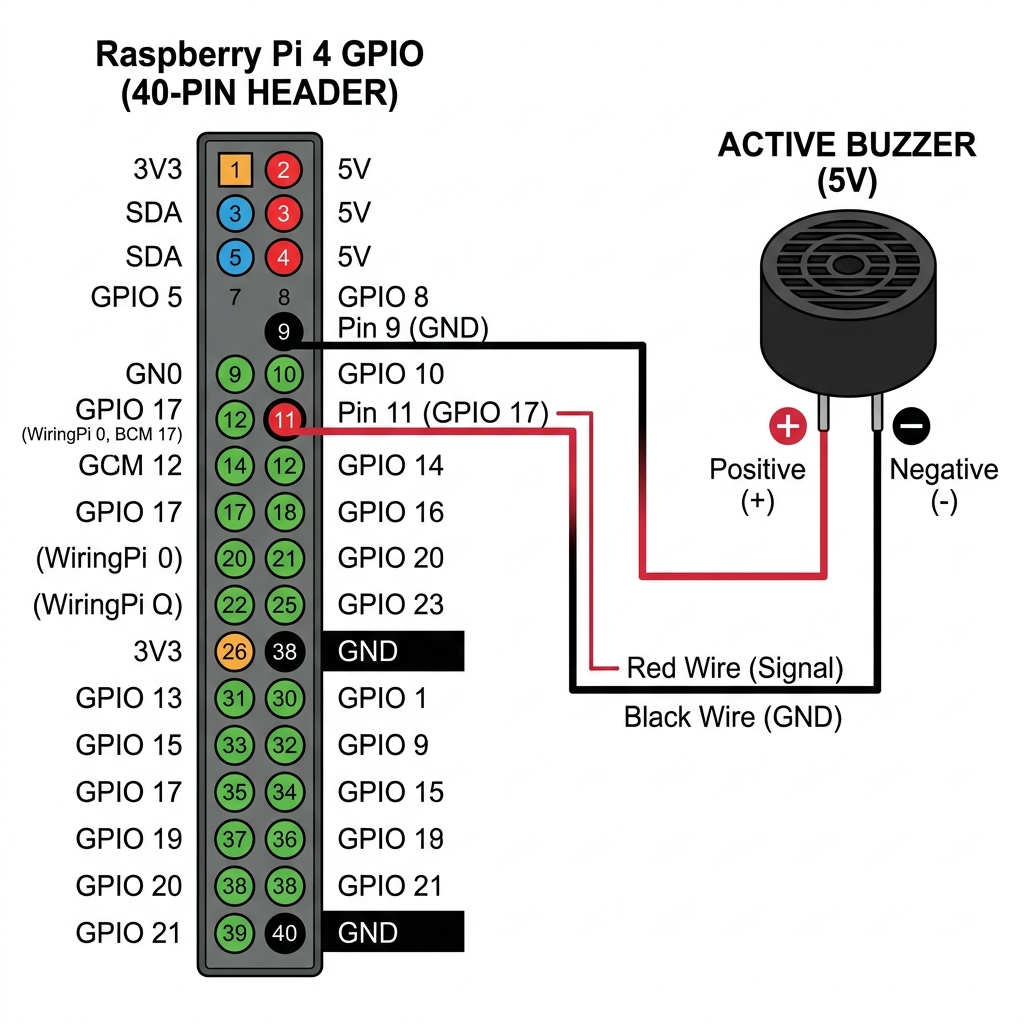
\includegraphics[width=0.65\textwidth]{images/rpi_buzzer_wiring.png}
    \caption{Schéma de branchement physique du buzzer actif sur le port GPIO du Raspberry Pi 4}
    \label{fig:rpi-wiring}
\end{figure}

Comme illustré par la figure \ref{fig:rpi-wiring}, la borne positive du buzzer est câblée sur la broche physique 11 (GPIO 17 en numérotation logique BCM) et la borne négative sur la broche physique 9 qui fournit la masse commune (GND). L'état logique de la broche GPIO 17 contrôle directement l'activation sonore :
\begin{itemize}
    \item \textbf{État Bas (LOW / 0 V) :} Le buzzer est éteint et silencieux.
    \item \textbf{État Haut (HIGH / 3.3 V) :} Le buzzer est alimenté et émet un son continu à pleine puissance.
\end{itemize}

\subsection{Architecture Logicielle et Programmation Concurrente (Multithreading)}

Pour assurer un fonctionnement fluide de l'IHM et une réactivité optimale du matériel en temps réel, le script Python autonome \texttt{icem\_station.py} utilise une architecture multithread (programmation concurrente). Cette structure évite que les requêtes réseau vers Firebase ou les temporisations logicielles pour faire clignoter le buzzer ne bloquent l'interface utilisateur.

Trois processus légers (threads) s'exécutent de manière asynchrone et partagent le même contexte de mémoire :

\begin{enumerate}
    \item \textbf{Thread Principal (IHM - Tkinter) :} Il gère l'affichage graphique à l'aide de la bibliothèque native \texttt{tkinter}. Pour transformer l'écran en un pupitre industriel hermétique masquant le système d'exploitation Linux, la fenêtre Tkinter est configurée en mode Kiosque avec les paramètres \texttt{fullscreen = True} et \texttt{topmost = True}. Ce thread capture également les événements tactiles de l'opérateur (tels que la validation tactile de la résolution d'une anomalie).
    \item \textbf{Thread d'Écoute Firebase Realtime Database (Service Firebase) :} Ce thread d'écoute en tâche de fond est géré par la bibliothèque \texttt{pyrebase} (un SDK tiers léger). Toutes les 2 secondes, il interroge le nœud \texttt{/active\_anomalies} de la base de données Firebase. Si des modifications de données sont détectées, il met à jour la structure interne et appelle la méthode \texttt{root.after()} pour notifier l'interface graphique Tkinter de manière \textit{thread-safe}.
    \item \textbf{Thread de Contrôle Sonore (Buzzer) :} Ce thread dédié est chargé de générer des bips intermittents en cas d'alerte active. Il exécute une boucle alternant l'écriture de l'état logique \texttt{HIGH} ($350\text{ ms}$) et \texttt{LOW} ($350\text{ ms}$) sur la broche GPIO 17, rythmée par des instructions \texttt{time.sleep(0.35)}. L'exécution dans un thread séparé évite de figer le reste de l'application pendant ces délais.
\end{enumerate}

Le diagramme de séquence simplifié ci-dessous décrit la communication asynchrone entre ces trois threads :

\begin{figure}[H]
\centering
\begin{verbatim}
+-----------------------+      +-----------------------+      +-----------------------+
|  Thread 2 : Firebase  |      |   Thread 1 : Tkinter  |      |   Thread 3 : Buzzer   |
+-----------------------+      +-----------------------+      +-----------------------+
            |                              |                              |
  [Polling 2 secondes]                     |                              |
  /active_anomalies                        |                              |
            |                              |                              |
  (Changement détecté)                     |                              |
            |---[ update_anomalies() ]---->|                              |
            |    (via root.after() GUI)    |                              |
            |                              |                              |
            |                              |---[ start_alert() ]--------->|
            |                              |                              | [Bips 350ms ON/OFF]
            |                              |<=-=[ Met à jour l'écran ]==  | (GPIO.output(17, HIGH))
            |                              |      (Fond rouge + Détails)  | (time.sleep(0.35))
            |                              |                              |
            |                              |                              |
            |                              | <Clic tactile "TRAITÉ">      |
            |                              |                              |
            |<--[ resolve_anomaly() ]------|                              |
            |    (Écrit dans RTDB)         |                              |
            |                              |                              |
  [Notification vide reçue]                |                              |
            |                              |                              |
            |---[ update_anomalies() ]---->|                              |
            |    (Aucune anomalie active)  |                              |
            |                              |                              |
            |                              |---[ stop_alert() ]---------->|
            |                              |                              | [Silence et GPIO LOW]
            |                              |<=-=[ Met à jour l'écran ]==  | (GPIO.output(17, LOW))
            |                              |      (Fond vert - Conforme)  |
            v                              v                              v
\end{verbatim}
\caption{Diagramme de communication et d'orchestration multithread de la station IoT}
\label{fig:multithread-diagram}
\end{figure}

\subsection{Implémentation Logicielle et Classes Principales}

Le script Python est entièrement structuré de manière orientée objet. Il comporte quatre classes principales chargées chacune d'une responsabilité spécifique dans le cycle de vie de l'application.

\subsubsection{La classe \texttt{BuzzerController} : Contrôle du matériel}

Cette classe encapsule l'accès aux broches matérielles à l'aide de la bibliothèque \texttt{RPi.GPIO}. Elle gère l'initialisation du GPIO de la carte en mode BCM, la configuration de la broche $17$ en sortie, et le thread de bips asynchrones.

\begin{lstlisting}[language=Python, caption=Structure de contrôle du buzzer dans icem\_station.py]
class BuzzerController:
    def __init__(self):
        self._thread = None
        self._stop_event = threading.Event()
        self._active = False

        if RUNNING_ON_PI:
            GPIO.setmode(GPIO.BCM)
            GPIO.setwarnings(False)
            GPIO.setup(BUZZER_PIN, GPIO.OUT)
            GPIO.output(BUZZER_PIN, GPIO.LOW)
            log.info(f"Buzzer initialisé sur GPIO {BUZZER_PIN}")
        else:
            log.info("Mode simulation PC activé")

    def _bip_loop(self):
        while not self._stop_event.is_set():
            self._set_buzzer(True)
            time.sleep(BIP_ON) # 350 ms ON
            self._set_buzzer(False)
            time.sleep(BIP_OFF) # 350 ms OFF

    def _set_buzzer(self, state: bool):
        if RUNNING_ON_PI:
            GPIO.output(BUZZER_PIN, GPIO.HIGH if state else GPIO.LOW)

    def start_alert(self):
        if self._active:
            return
        self._active = True
        self._stop_event.clear()
        self._thread = threading.Thread(target=self._bip_loop, daemon=True)
        self._thread.start()

    def stop_alert(self):
        if not self._active:
            return
        self._active = False
        self._stop_event.set()
        if self._thread:
            self._thread.join(timeout=2)
        self._set_buzzer(False)

    def cleanup(self):
        self.stop_alert()
        if RUNNING_ON_PI:
            GPIO.cleanup()
\end{lstlisting}

\subsubsection{La classe \texttt{FirebaseService} : Liaison de données temps réel}

Elle initialise la connexion vers la base de données Firebase Realtime Database à l'aide de Pyrebase et orchestre l'écoute en arrière-plan.

\begin{lstlisting}[language=Python, caption=Service Firebase utilisant Pyrebase dans icem\_station.py]
class FirebaseService:
    def __init__(self, callback):
        self._callback = callback
        self._active = False
        self._thread = None
        try:
            self._firebase = pyrebase.initialize_app(FIREBASE_CONFIG)
            self._db = self._firebase.database()
            log.info("Firebase connecté avec succès")
        except Exception as e:
            log.error(f"Erreur d'initialisation Firebase : {e}")
            sys.exit(1)

    def start_listening(self):
        self._active = True
        self._thread = threading.Thread(target=self._poll_loop, daemon=True)
        self._thread.start()

    def _poll_loop(self):
        previous_data = None
        while self._active:
            try:
                res = self._db.child("active_anomalies").get()
                data = res.val()
                if data != previous_data:
                    active = []
                    if data:
                        if isinstance(data, dict):
                            for doc_id, val in data.items():
                                active.append({"id": doc_id, **val})
                    # Tri chronologique des anomalies pour afficher la plus récente
                    active.sort(key=lambda x: x.get("detectedAt", ""), reverse=True)
                    self._callback(active)
                    previous_data = data
            except Exception as e:
                log.error(f"Erreur lors du sondage Firebase : {e}")
            time.sleep(2)

    def resolve_anomaly(self, anomaly_id: str):
        try:
            self._db.child("resolutions").child(anomaly_id).set({
                "statut": "traitee",
                "dateResol": datetime.now().isoformat()
            })
            return True
        except Exception as e:
            log.error(f"Erreur d'écriture de la résolution : {e}")
            return False
\end{lstlisting}

\subsubsection{La classe \texttt{WorkshopGUI} : Interface Homme-Machine}

Elle construit et gère l'aspect de l'IHM. En l'absence d'anomalie, elle affiche un écran vert uniforme (code hexadécimal \texttt{\#052e16}, vert sombre pour ne pas agresser les yeux des techniciens en atelier) signifiant \texttt{"PRODUCTION CONFORME"}.
Dès qu'une anomalie est notifiée par le service Firebase :
\begin{itemize}
    \item Le fond d'écran bascule en rouge sombre (\texttt{\#1a0000}) pour signaler visuellement le danger.
    \item Des bandeaux supérieur et inférieur de couleur rouge vif (\texttt{\#ef4444}) clignotent toutes les $700\text{ ms}$ (contrôlés par la fonction récursive Tkinter \texttt{\_blink\_tick()}).
    \item Une fiche d'information s'affiche dynamiquement au centre de l'IHM, présentant les métadonnées de l'anomalie : type de défaut, identifiant unique du câble défectueux, gravité, heure de détection et mode d'inspection (IA ou inspection manuelle).
    \item Un bouton tactile de grande taille \texttt{"MARQUER COMME TRAITÉ"} apparaît, obligeant l'opérateur à cliquer et à confirmer avant d'envoyer la commande de résolution dans Firebase RTDB.
\end{itemize}

\subsection{Déploiement Industriel : Automatisation Linux par Service Systemd}

Pour déployer la station de façon permanente en atelier sans exiger d'intervention humaine sur le système d'exploitation du Raspberry Pi lors de la mise sous tension, le script Python a été configuré sous forme de démon Linux à l'aide de l'utilitaire \texttt{systemd}.

Le fichier de configuration \texttt{icem\_station.service} a été écrit et copié dans le répertoire système \texttt{/etc/systemd/system/} :

\begin{lstlisting}[language=bash, caption=Fichier de configuration de service systemd (icem\_station.service)]
[Unit]
Description=ICEM Quality Control - Station d'Alerte Atelier (Firebase + GUI + Buzzer)
After=network-online.target graphical.target
Wants=network-online.target

[Service]
Type=simple
User=icem
Group=icem
# Variables d'environnement indispensables pour autoriser le service
# execute en arriere-plan a ouvrir une fenetre graphique sur l'ecran X11 (:0)
Environment=DISPLAY=:0
Environment=XAUTHORITY=/home/icem/.Xauthority

WorkingDirectory=/home/icem/Descktop/maram+riheme
ExecStart=/usr/bin/python3 /home/icem/Descktop/maram+riheme/icem_station.py

# Politique de redemarrage automatique en cas de crash
Restart=on-failure
RestartSec=10

StandardOutput=journal
StandardError=journal

[Install]
WantedBy=graphical.target
\end{lstlisting}

\subsubsection{Directives clés de systemd}
\begin{itemize}
    \item \textbf{\texttt{After=network-online.target graphical.target} :} Garantit que l'application ne s'exécute qu'une fois que la connexion réseau est établie (pour Firebase) et que le serveur d'affichage graphique X11 (l'interface bureau) est opérationnel.
    \item \textbf{\texttt{Environment=DISPLAY=:0} :} Indique à la bibliothèque Tkinter sur quel écran physique ouvrir la fenêtre. La valeur \texttt{:0} correspond au premier écran physique connecté (l'écran tactile HDMI de 7 pouces). Sans cela, systemd génère une erreur \texttt{no display name and no $DISPLAY environment variable} et plante.
    \item \textbf{\texttt{Restart=on-failure} et \texttt{RestartSec=10} :} Assure une résilience automatique en cas de défaillance logicielle ou de déconnexion réseau fatale, en redémarrant le script toutes les 10 secondes jusqu'à son rétablissement.
\end{itemize}

Les commandes d'administration système exécutées pour enregistrer, activer au démarrage du Raspberry Pi et lancer le service sont les suivantes :

\begin{lstlisting}[language=bash]
# Recharger la liste des services systemd apres copie du fichier .service
sudo systemctl daemon-reload

# Activer le service au demarrage automatique
sudo systemctl enable icem_station.service

# Demarrer le service immediatement
sudo systemctl start icem_station.service

# Consulter l'etat du service et verifier qu'il fonctionne correctement
sudo systemctl status icem_station.service
\end{lstlisting}

Ce déploiement garantit que si une coupure de courant survient dans l'atelier, la station d'alerte redémarre de manière entièrement autonome en moins de 45 secondes dès le retour de l'électricité, reprenant son écoute en tâche de fond et affichant son interface plein écran sans nécessiter de clavier ni de souris.
